\documentclass[UTF8]{ctexbeamer}	% Compile at least twice!
%\setbeamertemplate{navigation symbols}{}
\usetheme{Madrid}
% \setbeamertemplate{navigation symbols}{}
% \useinnertheme{rectangles}
% \useoutertheme{infolines}
% \useoutertheme[title,section,subsection=true]{smoothbars}
\useoutertheme{split}
\useinnertheme{rounded}
\setbeamertemplate{headline}{}
\usecolortheme{beaver}


% \usecolortheme{default}
% \usecolortheme{whale}
 
% -------------------
% Packages
% -------------------
\usepackage{
    amsmath,			% Math Environments
    amssymb,			% Extended Symbols
    enumerate,		    % Enumerate Environments
    graphicx,			% Include Images
    lastpage,			% Reference Lastpage
    multicol,			% Use Multi-columns
    multirow,			% Use Multi-rows
    pifont,			    % For Checkmarks
    stmaryrd,            % For brackets
    listings,
    subfigure,
}
\usepackage[english]{babel}
\usepackage{graphicx}
\usepackage{animate}
\usepackage{xeCJK}
\usepackage{fontspec} 
\setmainfont{Sarasa Gothic SC}
\setCJKmainfont{Sarasa Gothic SC}
% \setmainfont{Inconsolata}
% \setCJKmainfont{Inconsolata}
% \setmainfont{Microsoft YaHei}
% \setCJKmainfont{Microsoft YaHei}
% \setmainfont{Source Han Sans SC}
% \setCJKmainfont{Source Han Sans SC}

% \newfontfamily\os{Open Sans}
% \newfontfamily\oscl{Open Sans Condensed}
% \newfontfamily\tnr{Times New Roman}
% \newfontfamily\tnrc{Times New Roman Cyr}
% \newfontfamily\tim{Times}
% \newfontfamily\roc{Rockwell}
% \usepackage{CJK}
% \lstset{language=C++}
% \lstset{extendedchars=false}
% \lstset{breaklines}


% -------------------
% Colors
% -------------------
% \definecolor{UniOrange}{RGB}{212,69,0}
% \definecolor{UniGray}{RGB}{62,61,60}
% \definecolor{UniRed}{HTML}{B31B1B}
% \definecolor{UniGray}{HTML}{222222}
% \setbeamercolor{title}{fg=UniGray}
% \setbeamercolor{frametitle}{fg=UniOrange}
% \setbeamercolor{structure}{fg=UniOrange}
% \setbeamercolor{section in head/foot}{bg=UniGray}
% \setbeamercolor{author in head/foot}{bg=UniGray}
% \setbeamercolor{date in head/foot}{fg=UniGray}
% \setbeamercolor{structure}{fg=UniOrange}
% \setbeamercolor{local structure}{fg=black}
% \beamersetuncovermixins{\opaqueness<1>{0}}{\opaqueness<2->{15}}


% -------------------
% Fonts & Layout
% -------------------
% \usepackage{palatino}
\usefonttheme{serif}
% \setbeamerfont{title like}{shape=\scshape}
% \setbeamerfont{frametitle}{shape=\scshape}
% \setbeamertemplate{itemize items}[circle]
% \setbeamertemplate{enumerate items}[default]


% -------------------
% Commands
% -------------------

% Special Characters
% \newcommand{\N}{\mathbb{N}}
% \newcommand{\Z}{\mathbb{Z}}
% \newcommand{\Q}{\mathbb{Q}}
% \newcommand{\R}{\mathbb{R}}
%\newcommand{\C}{\mathbb{C}}

% Math Operators
% \DeclareMathOperator{\im}{im}
% \DeclareMathOperator{\Span}{span}

% Special Commands
% \newcommand{\pf}{\noindent\emph{Proof. }}
% \newcommand{\ds}{\displaystyle}
% \newcommand{\defeq}{\stackrel{\text{def}}{=}}
% \newcommand{\ov}[1]{\overline{#1}}
% \newcommand{\ma}[1]{\stackrel{#1}{\longrightarrow}}
% \newcommand{\twomatrix}[4]{\begin{pmatrix} #1 & #2 \ #3 & #4 \end{pmatrix}}


% -------------------
% Tikz & PGF
% -------------------
\usepackage{tikz}
\usepackage{tikz-cd}
\usetikzlibrary{
    calc,
    decorations.pathmorphing,
    matrix,arrows,
    positioning,
    shapes.geometric
}
\usepackage{pgfplots}
\pgfplotsset{compat=newest}
\usepackage{wrapfig}
\usepackage{cite}


% -------------------
% Theorem Environments
% -------------------
\usepackage{amsthm}
\theoremstyle{plain}
\newtheorem{sit}{Situation}[section]
\newtheorem{prop}{Proposition}[section]
\newtheorem{rtm}{Theorem}[section]
\newtheorem{cor}{Corollary}[section]
\theoremstyle{definition}
\newtheorem{das}{Data structure}[section]
\newtheorem{nex}{Non-Example}[section]
\newtheorem{cla}{class}[section]
\newtheorem{emt}{}[section]
\newtheorem{defn}{Definition}[section]
\theoremstyle{remark}
\newtheorem{rem}{Remark}[section] 
\numberwithin{equation}{section}

\newcommand\caesura{$\mkern -8.5mu\raise -.2ex\hbox{\rotatebox[]{180}{\`}}\ $}
\setbeamertemplate{caption}[numbered]
% -------------------
% Title Page
% -------------------
\title{\textcolor{red}{三维 YinSet 中的表示一致与容忍度设置}}
%\subtitle{\textcolor{white}{Mathematics Conference for the Mysterious and dMagical}}  
\author{邱云昊, 谭焱 
% \newline \newline
%  \small{硕士导师: 王何宇\, \\
%  申请博士导师: 张庆海}
 }

% \institute{\small{现硕士导师: 王何宇 、张庆海 \newline 拟转博士指导教师: 张庆海} \newline   \newline 浙江大学数学科学学院}
\date{\today} 


% -------------------
% Content
% -------------------
\begin{document}
% \begin{CJK}{GBK}{kai}

% Title Page
\begin{frame}
    \titlepage
\end{frame}


\begin{frame}
    \frametitle{提纲}
    \tableofcontents
\end{frame}

\section{背景}

% \subsection{\textcolor{red}{}}
\begin{frame}
    \frametitle{背景}
    \begin{itemize}
        \item 已有一个表示和计算YinSet的布尔运算程序.
        \item 现有程序要求输入是合法的YinSet表示:
              \begin{enumerate}
                  \item 没有且不能检测输入数据是否唯一表示YinSet.
                  \item 不能将非法YinSet表示数据修正为合法YinSet唯一表示.
              \end{enumerate}
        \item 表示YinSet边界的三角形畸形, 影响边界表示的质量.
    \end{itemize}
    \begin{columns}
        \column{0.4\linewidth}<1->
        \centering
        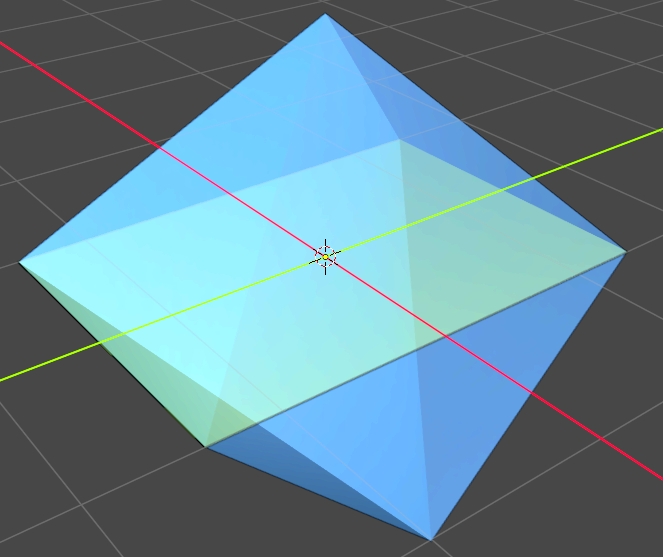
\includegraphics[width = .6\textwidth]{fig/wrong5em.png}
        \column{0.6\linewidth}<1->
        \centering
        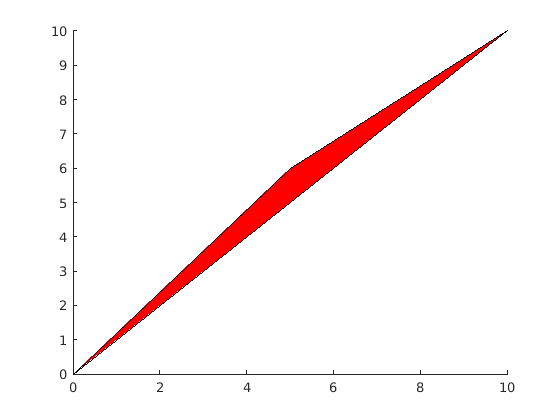
\includegraphics[width = .6\textwidth]{fig/illTri.png}
    \end{columns}
\end{frame}


% \begin{frame}
%     \frametitle{二维殷集}
%     \begin{itemize}
%         \item \textcolor{red}{殷集}:边界有界的正则半解析开集.所有殷集构
%               成的集合被称为殷空间,记为 $\mathbb{Y}$.
%         \item 二维空间中,任一个殷集可以唯一表示为
%               \[\mathcal{Y} = \cup_j^{\bot \bot}\cap_i \text{int}(\gamma_{j, i} ),\]
%               约当曲线 $\gamma_{j, i}$是$\mathcal{Y}$内第$j$个连通分量
%               的第$i$条边界.
%         \item 实现了殷集上的布尔代数.
%     \end{itemize}
%     \begin{figure}[!htb]
%         \centering
%         \subfigure{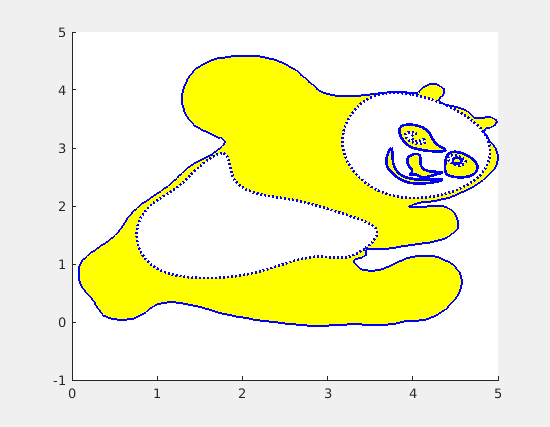
\includegraphics[width=0.3\textwidth]{fig/p.png}}
%         \subfigure{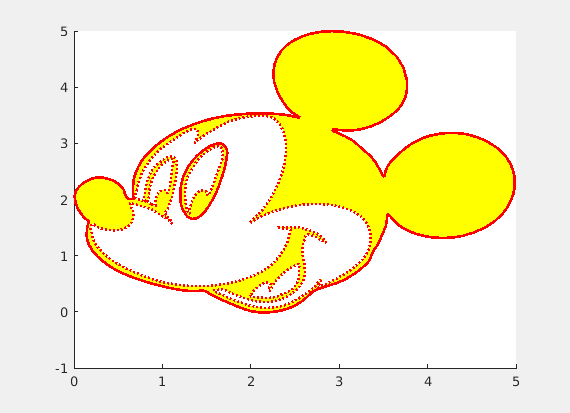
\includegraphics[width=0.3\textwidth]{fig/m.png}}
%         \subfigure{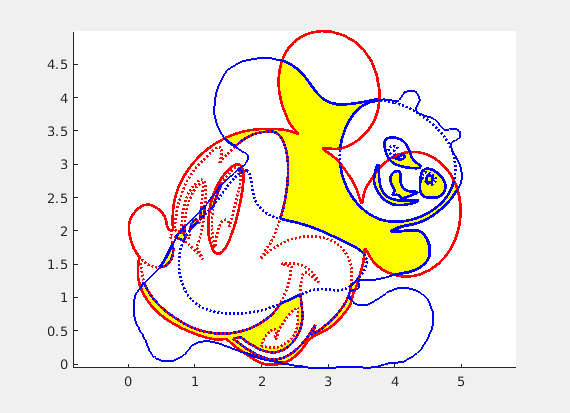
\includegraphics[width=0.3\textwidth]{fig/pm.png}}
%         \caption{二维殷集的交}
%         %   \vspace{0.2in}
%     \end{figure}
% \end{frame}

% \begin{frame}
%     \frametitle{黏合紧曲面}
%     \begin{itemize}
%         \item
%               \textcolor{red}{二流形的分类定理} \newline
%               有向的二维紧流形同胚于球面或轮胎面或轮胎面的连通和.
%               \begin{figure}[!htb]
%                 \centering
%                 \subfigure{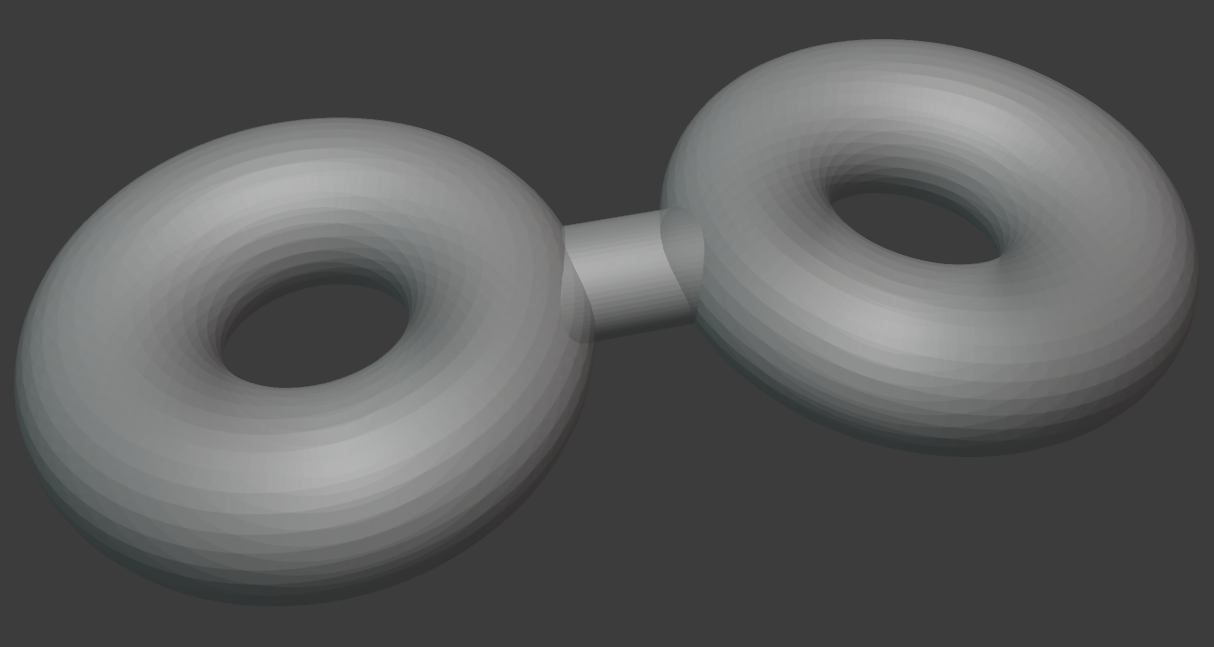
\includegraphics[width=0.4\textwidth]{fig/connectsum.png}} \qquad
%                 \subfigure{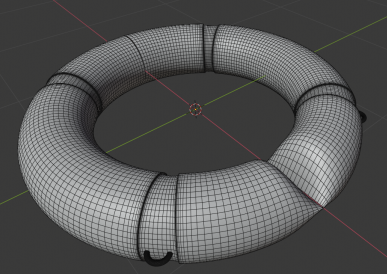
\includegraphics[width=0.3\textwidth]{fig/past.png}}
%             \end{figure}


%         \item 黏合紧曲面是一个二维连通紧流形或这种流形的商空间, 其商映射
%               将紧流形与一维 CW 复形同胚的子集粘在一起; 将这个一维子集删除后
%               该黏合紧曲面仍然是连通的.
%     \end{itemize}
% \end{frame}

% \begin{frame}
%     \frametitle{三维殷集的唯一表示}
%     \begin{itemize}
%         \item 任一个殷集$\mathcal{Y} \in \mathbb{Y}$可以唯一表示为
%               \[\mathcal{Y} = \cup_j^{\bot \bot} \cap_i \text{int}(\Gamma_{j, i}),\]
%               黏合紧曲面$\Gamma_{j, i}$是$\mathcal{Y}$的第$j$个连通分量的第$i$个边界.
%         \item 连通分量个数等于正向黏合紧曲面的个数(有界殷集)或正向黏合紧曲面个数+1(无界殷集).

%         \item 洞的个数等于负向黏合紧曲面的个数.
%     \end{itemize}
%     \begin{columns}
%         \column{0.35\linewidth}<1->
%         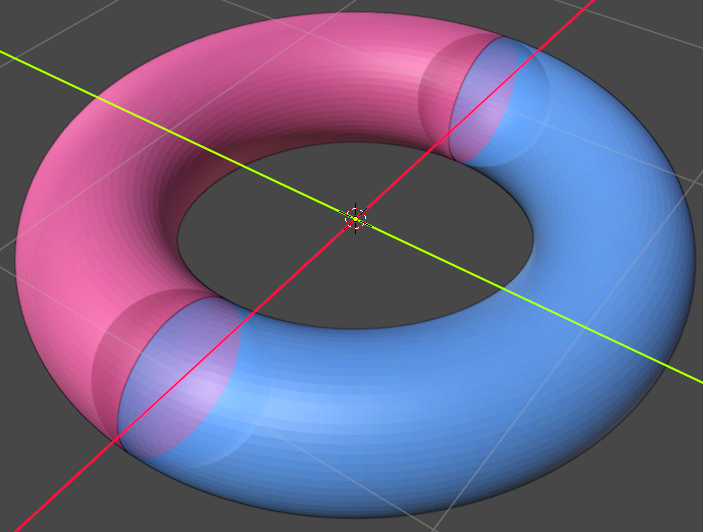
\includegraphics[width = \textwidth]{fig/ys1.png}
%         \column{0.35\linewidth}<1->
%         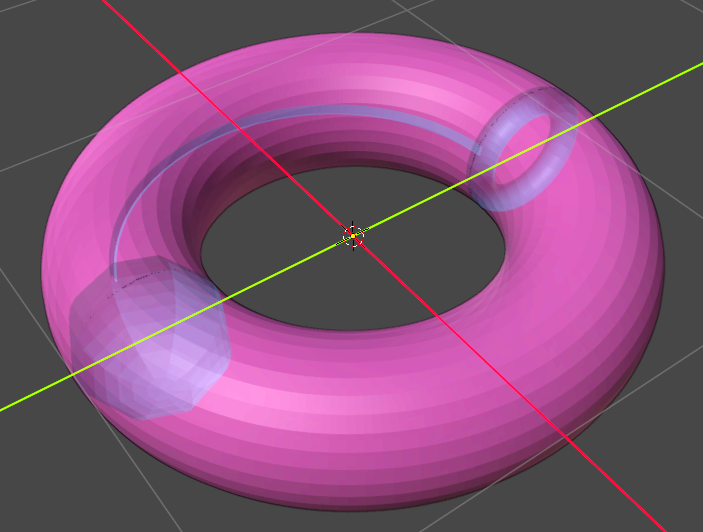
\includegraphics[width = \textwidth]{fig/ys5.png}
%     \end{columns}
% \end{frame}

\section{YinSet表示数据处理}
\begin{frame}
    \frametitle{实现步骤}
    \begin{itemize}
        \item 检验且改造非法输入数据.
    \begin{enumerate}
        \item 非闭合曲面的处理.
        \item 曲面的定向处理.
        \item 恰当交和重合处理.
        \item 包含关系处理.
    \end{enumerate}

        \item 提高网格质量.
        \begin{enumerate}
            \item 设定边长上下界和三角形面积下界.
            \item 过短和过长边处理.
            \item 面积过小三角形处理.
        \end{enumerate}
    \end{itemize}
\end{frame}

\subsection{改造非法输入数据}
\begin{frame}
    \frametitle{非闭合曲面处理}
    \begin{itemize}
        \item 三角网格表示的曲面闭合当且仅当\textcolor{red}{每条边相邻
        偶数个三角形}.

        \item 所有相邻奇数个三角形的边无法恰当粘合成闭合曲面.
        
        \item 沿相邻奇数个三角形的边剪开必得到一些曲面片和闭合曲面.
        
        \item 如下图,无法简易判断应该删除或者填补曲面片, 用户结合
        图形界面恰当的填补或删除曲面片.
        
    \end{itemize}

    \begin{columns}
        \column{0.5\linewidth}<1->
        \centering
        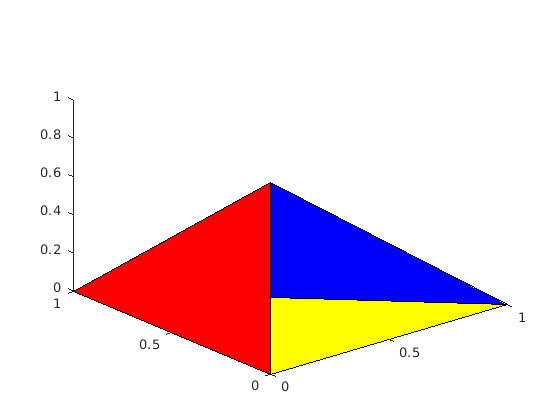
\includegraphics[width = .8\textwidth]{fig/bound1.png}
        \column{0.5\linewidth}<1->
        \centering
        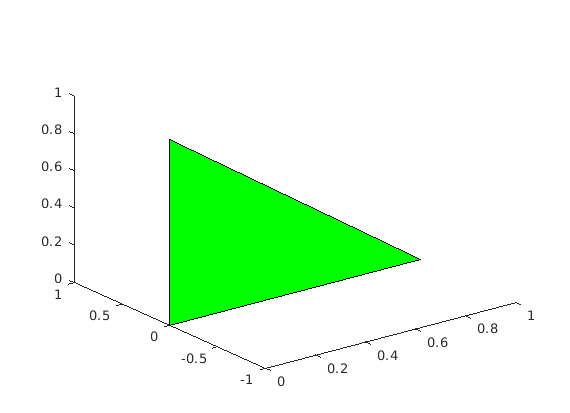
\includegraphics[width = .8\textwidth]{fig/bound2.png}
    \end{columns}
\end{frame}

\begin{frame}
    \frametitle{曲面的定向处理}
    \begin{itemize}
        \item 闭合曲面将空间划分的内部和外部.

        \item 三角形的法向量指向外部空间.
        
        \item 相邻两个三角形的边在两个三角形中方向相反.
        
        \item 相邻超过两个三角形的边, 局部将空间
        划分为内部和外部.

        \item 改造数据需要用户给定闭合曲面有界或无界.
        
    \end{itemize}
    \begin{columns}
        \column{0.5\linewidth}<1->
        \centering
        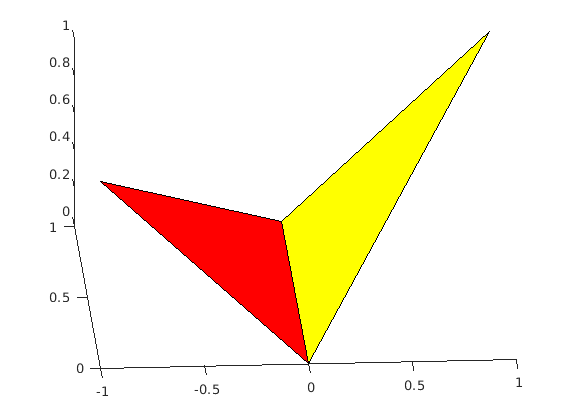
\includegraphics[width = .8\textwidth]{fig/nearTri1.png}
        \column{0.5\linewidth}<1->
        \centering
        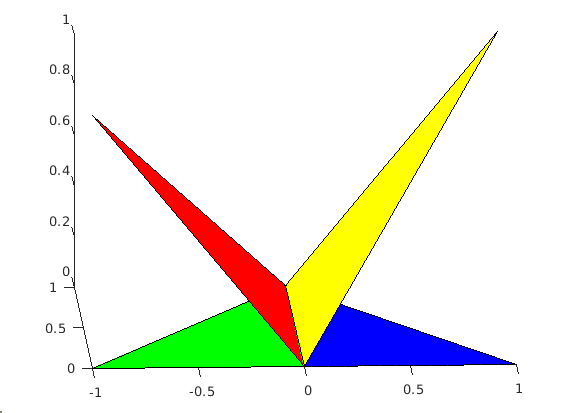
\includegraphics[width = .8\textwidth]{fig/nearTri2.png}
    \end{columns}
\end{frame}


\begin{frame}
    \frametitle{恰当交和重合处理}
    \begin{itemize}
        \item 黏合紧曲面之间没有恰当交或重合.

        \item 通过YinSet布尔运算改造曲面.
        
        \item 需要用户决定求交, 求并或移除曲面.
        \begin{enumerate}[1]
            \item 如左图所示, 当都内部有界或无界时,
            选取求并或者求交恰当.
            \item 如右图所示, 两个长方形方向相反时, 
            需要根据方向选取求交或求并保留大部分边界信息.
        \end{enumerate}
    \end{itemize}
    \begin{columns}
        \column{0.5\linewidth}<1->
        \centering
        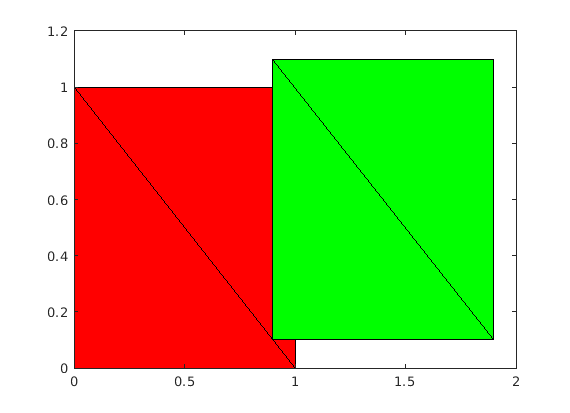
\includegraphics[width = .8\textwidth]{fig/rectangle1.png}
        \column{0.5\linewidth}<1->
        \centering
        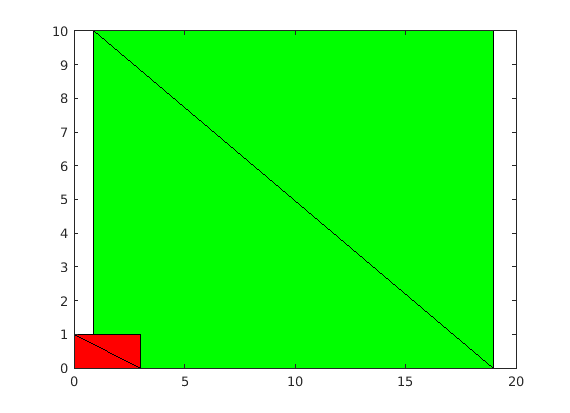
\includegraphics[width = .8\textwidth]{fig/rectangle2.png}
    \end{columns}
\end{frame}

\begin{frame}
    \frametitle{包含关系处理}
    \begin{itemize}
        \item YinSet边界将空间划分为内部和外部.

        \item 直接包含的黏合紧曲面之间的空间是连通的.
        
        \item 用户给定YinSet内部有界或无界后确定所有
        曲面的方向.
    \end{itemize}
    \begin{columns}
        \column{0.5\linewidth}<1->
        \centering
        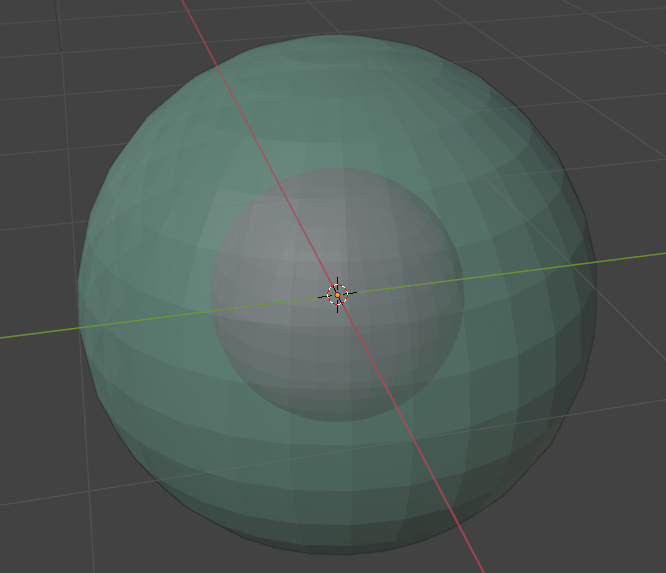
\includegraphics[width = .8\textwidth]{fig/faceContain.png}
    \end{columns}
\end{frame}

\subsection{优化三角网格}
\begin{frame}
    \frametitle{设置三角网格的要求}
    \begin{itemize}
        \item 为三角网格表示精度要求三角形边长上界为$h_L$.
        \item 因希望三角网格均匀, 设置边长下界为$r_{tiny}h_L$.
        \item 从三角网格拟合曲面的需要, 杜绝畸形包含角度过小的三角形,从
        \[ \sin \angle ABC =  S_{ABC} / \left\| AB \right\| \cdot \left\| BC \right\|. \]
        设置三角形面积下界$S_{min}$.
        
    \end{itemize}
\end{frame}

\begin{frame}
    \frametitle{满足三角网格的边长需求}
    \begin{itemize}
    \item 过长边取中点分割.
    \item 过长边用中点代替边的两个端点.
    \begin{columns}
        \column{.6\linewidth}<1->
        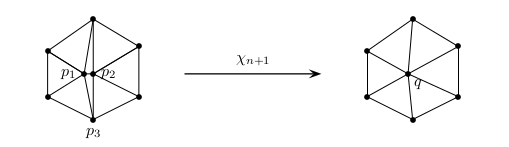
\includegraphics[width = \textwidth]{fig/combinePoint.png}
     \end{columns}
     \item 必可在有限步后使得不存在过长或过短的边.
    \end{itemize}
    
\end{frame}


\begin{frame}
    \frametitle{处理面积过小的三角形}
    \begin{itemize}
        \item 交换对角线.
        \begin{columns}
            \column{.6\linewidth}<1->
            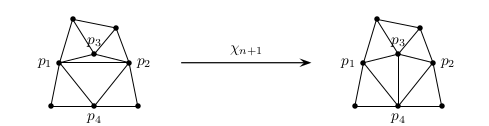
\includegraphics[width = \textwidth]{fig/swapcross.png}
         \end{columns}
        \item 局部重新三角化.
        \begin{columns}
            \column{.25\linewidth}<1->
            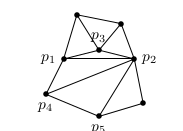
\includegraphics[width = \textwidth]{fig/reTriangule.png}
         \end{columns}
    \end{itemize}
\end{frame}

\subsection{气泡充填法}
\begin{frame}
    \frametitle{启发来源}
    \begin{itemize}
        \item 数量充足的气泡会均匀填充整个空间.
        \begin{columns}
            \column{.8\linewidth}<1->
            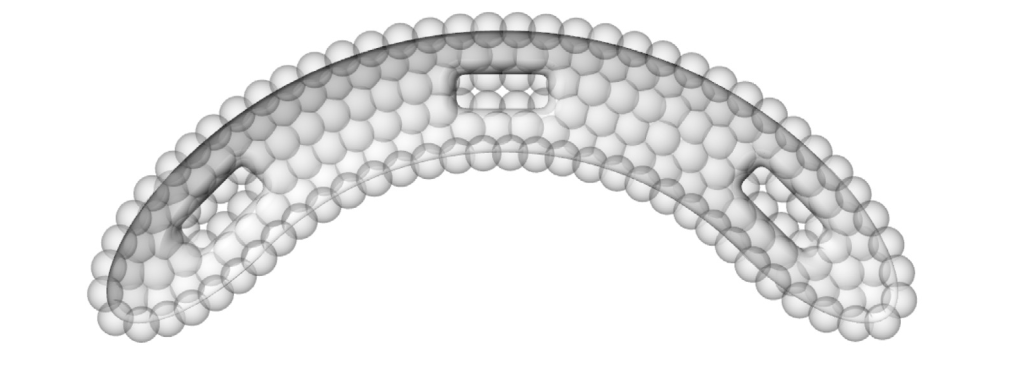
\includegraphics[width = \textwidth]{fig/bubble.png}
         \end{columns}
        \item 将空间限制在曲面上, 以每个三角形顶点为气泡中心, 给定恰当的
        质量, 斥力和阻力.

        \item 充足的顶点情况下, 有限步后的平衡态时三角形顶点均匀分布在
        YinSet边界上.
    \end{itemize}
\end{frame}

\begin{frame}
    \frametitle{恰当的顶点数量}
        \begin{itemize}
            \item 设$l_0 \in [r_{tiny}h_L, h_L]$为期望的边长.
            \item 边长为$l_0$的等边三角形面积为$\frac{\sqrt{3}}{4} l_0^2$.
            \item 依据原面积$A$和期望面积计算填充顶点数量
            \[n = \frac{2 \sqrt{3} A}{3 l_0^2}. \]
            \begin{columns}
                \column{.4\linewidth}<1->
                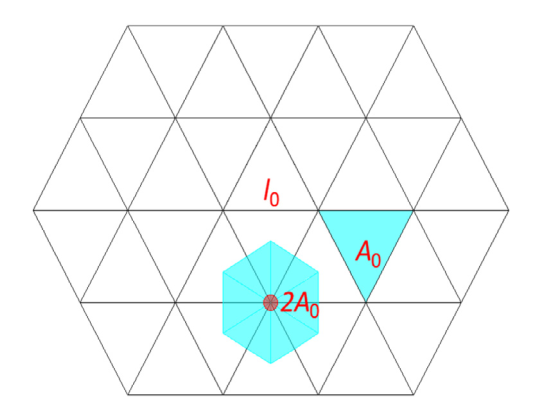
\includegraphics[width = \textwidth]{fig/nodeNumber.png}
             \end{columns}
        \end{itemize}
\end{frame}

\begin{frame}
    \frametitle{顶点之间的斥力}
    \begin{itemize}
      \item 定义顶点$p_i, p_j$之间的斥力
      \begin{equation}
        \label{equ:Tij}
        {\mathop{T}\limits^{\rightarrow}}_{ij} =
        \left\{ \begin{aligned}
            &k_b \cdot \left( R_i + R_j - \left| {\mathop{d}\limits^{\rightarrow}}_{ij} \right| \right) \cdot \frac{{\mathop{d}\limits^{\rightarrow}}_{ij}}{\left| {\mathop{d}\limits^{\rightarrow}}_{ij} \right|},\, &\left| {\mathop{d}\limits^{\rightarrow}}_{ij} \right| <  R_i + R_j ,\\
            &\,0,&\left| {\mathop{d}\limits^{\rightarrow}}_{ij} \right| \ge  R_i + R_j
      ,    \end{aligned}\right.
      \end{equation}
        \item 顶点$p_i$受到的斥力和
        \begin{equation}
            \label{equ:Ti}
            {\mathop{T}\limits^{\rightarrow}}_{i} =
           \left\{ \begin{aligned}
                &{\sum\limits^{n+m}_{j=1,j\neq i}} {\mathop{T}\limits^{\rightarrow}}_{ji},\, &\text{第i个质点是随机生成的点,}\\
                &\,\mathop{0}\limits^{\rightarrow},&\text{第i个质点是空间多边形的顶点,}
             \end{aligned}\right.
          \end{equation}

          \item 弹性系数和作用半径$k_b, R_i$是影响系统最终效果的
          重要参数.
            \end{itemize}
\end{frame}

\begin{frame}
    \frametitle{运动阻力}
        \begin{itemize}
            \item 为降低系统能量达到最终的平衡态.
            \item 顶点$p_i$受到的运动阻力
            \begin{equation}
                \label{equ:fi}
              {\mathop{f}\limits^{\rightarrow}}_{i} = -k_f\cdot {\mathop{v}\limits^{\rightarrow}}_{i},
              \end{equation}

              \item 顶点$p_i$所受的最终合力 
              \begin{equation}
                \label{equ:Fi}
                {\mathop{F}\limits^{\rightarrow}}_{i} = {\mathop{T}\limits^{\rightarrow}}_{i} + {\mathop{f}\limits^{\rightarrow}}_{i},
              \end{equation}
        \end{itemize}
\end{frame}

\begin{frame}
    \frametitle{迭代方程}
        \begin{itemize}
            \item 随机给定$n$个顶点的初始位置和初始速度$\mathop{0}\limits^{\rightarrow}$.
            \item 顶点$p_i$的位置,速度迭代方程
            \begin{equation}
                \label{equ:visi}
                \begin{aligned}
                &  {\mathop{v}\limits^{\rightarrow}}_{i}(t+k) = {\mathop{v}\limits^{\rightarrow}}_{i}(t) + \frac{{\mathop{F}\limits^{\rightarrow}}_{i}(t)}{m}k,\\
                 & {\mathop{s}\limits^{\rightarrow}}_{i}(t+k) = {\mathop{s}\limits^{\rightarrow}}_{i}(t) + \frac{{\mathop{v}\limits^{\rightarrow}}_{i}(t) + {\mathop{v}\limits^{\rightarrow}}_{i}(t+k)}{2}k,
                  \end{aligned}
              \end{equation}

              \item 当所有顶点最大位移充分小时迭代终止.
        \end{itemize}
\end{frame}

\begin{frame}
    \frametitle{重新三角化流程}
        \begin{itemize}
            \item 重新三角化区域通过面积过小三角形沿边拓展找出.
            \item 拓展时保持YinSet边界的非流形点始终在区域边界上.
            \item 区域中随机生成顶点后迭代.
            \item 得到顶点集后使用Delaunay三角化.
            \item 定义沿边传导的弹性斥力和拉力迭代调整顶点位置.
            \item 若结果违反边长面积要求, 返回第一步
            继续拓展重新三角化区域.
        \end{itemize}
\end{frame}

\section{存在的问题}
    \begin{frame}
        \frametitle{存在的问题}
    \begin{itemize}
        \item 无法建立气泡充填法的结果和参数之间的数学关系.
        \item $k_b, k_f$等参数的选择.
        \item 不能证明必定有限步后三角网格满足边长和面积条件.
    \end{itemize}
    \begin{columns}
        \column{.8\linewidth}<1->
        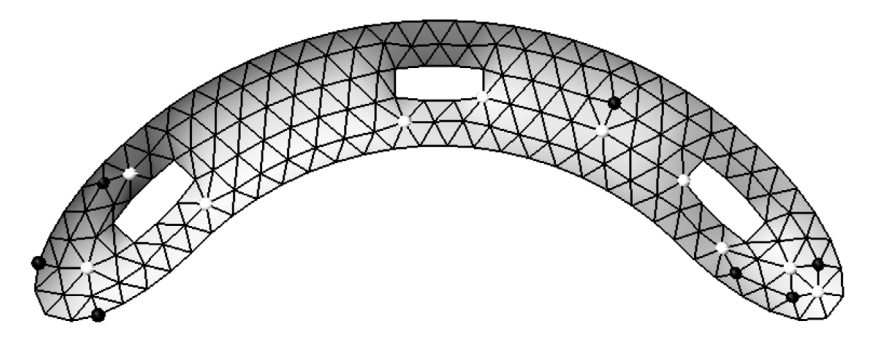
\includegraphics[width = \textwidth]{fig/weakness.png}
     \end{columns}

\end{frame}

\begin{frame}
    \centering\huge
    \textcolor{red}{请老师同学批评指正!}
\end{frame}
\end{document}